\documentclass{ximera}

\input{../preamble}
\author{Ivo Terek}
\license{Creative Commons Attribution-ShareAlike 4.0 International License}
\acknowledgement{}

\title{The Famous Function $f(x)=1/x$}

\begin{document}
\begin{abstract}
  
\end{abstract}
\maketitle


%\typeout{************************************************}
%\typeout{Motivating Questions}
%\typeout{************************************************}

\begin{motivatingQuestions}
\item What is a possible explanation, in terms of functions, for the fact that one cannot divide by zero? 
\item Are sine, cosine, and tangent really the only relevant trigonometric functions? Are there others? If so, how to understand them?
\end{motivatingQuestions}


%\typeout{************************************************}
%\typeout{Subsection Introduction}
%\typeout{************************************************}

\section{Introduction}

We know that if $a$ and $b$ are two real numbers, then $a/b$ makes sense, as long as $b$ is not equal to zero. Let's look at what happens when we make divisions by numbers very close to zero, but not equal to zero. Take $a=1$ for simplicity.

\begin{align*}
  \frac{1}{0.1} &= 10 \\ \frac{1}{0.01} &= 100 \\ \frac{1}{0.001} &= 1000 \\ \frac{1}{0.0001} &= 10000
\end{align*}

This pattern makes us want to say that $1/0$ equals to $+\infty$ (whatever $+\infty$ means, at this point), but this doesn't work. To understand why, let's consider divisions by numbers very close to zero, but this time negative. 

\begin{align*}
  \frac{1}{-0.1} &= -10 \\ \frac{1}{-0.01} &= -100 \\ \frac{1}{-0.001} &= -1000 \\ \frac{1}{-0.0001} &= -10000
\end{align*}

The same reasoning as before would tempt us to say that $1/0$ equals $-\infty$. And this raises the question of whether $\infty$ or $-\infty$ is the better choice. While on an instinctive psychological level we could think that $+\infty$ is better than $-\infty$, there's really no way to decide\footnote{Algebraically, the explanation is simple: if one could make sense of $1/0$ and say that equals some number $c$, then this would give $1 = 0 \cdot c$, so $1 = 0$ --- which is a complete collapse of the number system we have to deal with in our daily lives. But this doesn't give intuition for what is going on.} --- and this turns out to be related to the concept of \emph{limit}, which you'll learn in Calculus.

\section{Graph and asymptotics}

To continue our discussion in a more precise way, let's consider the function $f$, defined for all real numbers \emph{except for zero}, given by $f(x) = 1/x$. This is a very famous function, particularly useful as the building block for \emph{rational functions}, which we'll discuss soon. Note that essentially what we have just done in the introduction was to consider the values $$   f(0.1), f(0.01), f(0.001), \mbox{ and } f(0.0001),$$as well as $$f(-0.1), f(-0.01), f(-0.001), \mbox{ and } f(-0.0001).  $$
To get a good idea of the behavior a function has, our main strategy so far has been to just consider its graph. Naturally, plugging a handful of values won't cut it. Let's see what happens when we go to the other extreme and make divisions by very large numbers:

\begin{align*}
  \frac{1}{10} &= 0.1 \\ \frac{1}{100} &= 0.01 \\ \frac{1}{1000} &= 0.001 \\ \frac{1}{10000} &= 0.0001
\end{align*}

And from the negative side:

\begin{align*}
  \frac{1}{-10} &= -0.1 \\ \frac{1}{-100} &= -0.01 \\ \frac{1}{-1000} &= -0.001 \\ \frac{1}{-10000} &= -0.0001
\end{align*}


Here's what the graph looks like.


\begin{image}
\begin{tikzpicture}
    \begin{axis}
      \addplot[samples=200,domain=0.01:7]{1/x};
      \addplot[samples=200,domain=-7:-0.01]{1/x};
    \end{axis}
\end{tikzpicture}
\end{image}


% \begin{image}
% \begin{tikzpicture}
%                     \begin{axis}[]
%                         \addplot+[domain=-6.29:-0.001] {1/x}; \addplot+[domain=0.001:6.29]{1/x}
%                     \end{axis}
%                 \end{tikzpicture}
% \end{image}

% [IS THIS A BUILT-IN MACRO? PROBLEM WITH 0 OUTSIDE DOMAIN]


Here's what we can immediately see from the graph, confirming our intuition from the several divisions previously done:

\begin{callout}
  {\bf Asymptotics of $1/x$.}
  \begin{itemize}
  \item If $x \to +\infty$, then $1/x \to 0$ (reads ``when $x$ tends to $+\infty$, $1/x$ tends to $0$'').
  \item If $x \to 0^+$, then $1/x \to +\infty$ (reads ``when $x$ tends to zero from the right, $1/x$ tends to $+\infty$'').
  \item If $x \to 0^-$, then $1/x \to -\infty$ (reads ``when $x$ tends to zero from the left, $1/x$ tends to $-\infty$'').
  \item If $x \to -\infty$, then $1/x \to 0$ (reads ``when $x$ tends to $-\infty$, $1/x$ tends to $0$'').
  \end{itemize}
\end{callout}

We say that the line $x=0$ is a \emph{vertical asymptote} for $f(x) = 1/x$, while the line $y=0$ is a \emph{horizontal asymptote}. We will discuss asymptotes of rational functions in general in the next unit. Next, as far as symmetries go, we can see that the graph is symmetric about the line $y=x$:

\begin{image}
\begin{tikzpicture}
    \begin{axis}
      \addplot[samples=200,domain=0.01:7]{1/x};
      \addplot[samples=200,domain=-7:-0.01]{1/x};
      \addplot[dashed,samples=200,domain=-7:7]{-x};
    \end{axis}
\end{tikzpicture}
\end{image}

This indicates that $f(x) = 1/x$ is an odd function. You can also see this algebraically via $$  f(-x) = \frac{1}{-x} = -\frac{1}{x} = -f(x).  $$
By the way, the graph of $f(x) = 1/x$ is called a \emph{hyperbola}.

\section{Application: Reciprocals of trigonometric functions}

It turns out that applying $f$ to some famous functions, such as the usual trigonometric functions sine, cosine, and tangent, usually produces new interesting functions which can help to model several situations in a perhaps simpler way. Or, in other words, reciprocals of famous or useful functions also deserve some of our attention.

\begin{definition}
  The \emph{cosecant}, \emph{secant} and \emph{cotangent} functions are defined, respectively, by $$   \csc x = \frac{1}{\sin x}, \quad \sec x = \frac{1}{\cos x} \quad\mbox{and}\quad \cot x = \frac{1}{\tan x}.  $$
\end{definition}

\begin{example}
  Let's look at the cosecant function in more detail. We know that the expression $1/\sin(x)$ will be undefined whenever $\sin(x) = 0$. Recall that this happens when $x$ is one of the values in the infinite list $$   \ldots, -3\pi, -2\pi, -\pi, 0, \pi, 2\pi, 3\pi, \ldots   $$You can see this on the graph of the sine function:

  \begin{image}
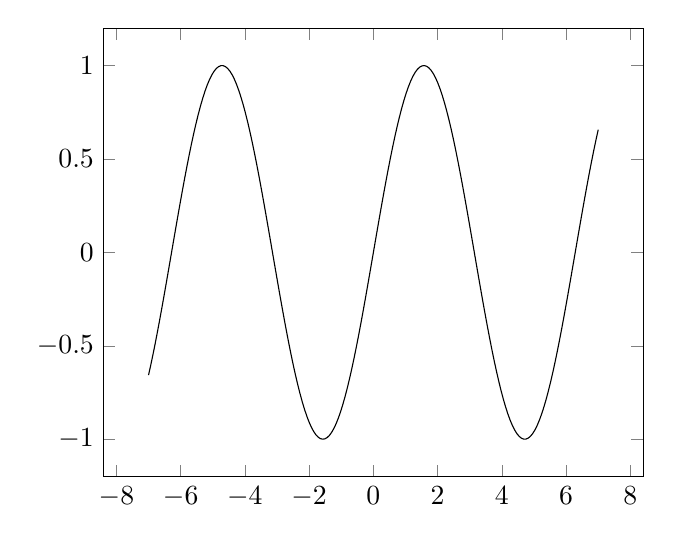
\begin{tikzpicture}
    \begin{axis}
      \addplot[samples=200,domain=-7:7]{sin(deg(x))};
    \end{axis}
\end{tikzpicture}
\end{image}

This means that such values make the cosecant function undefined. Here's its graph:

\begin{image}
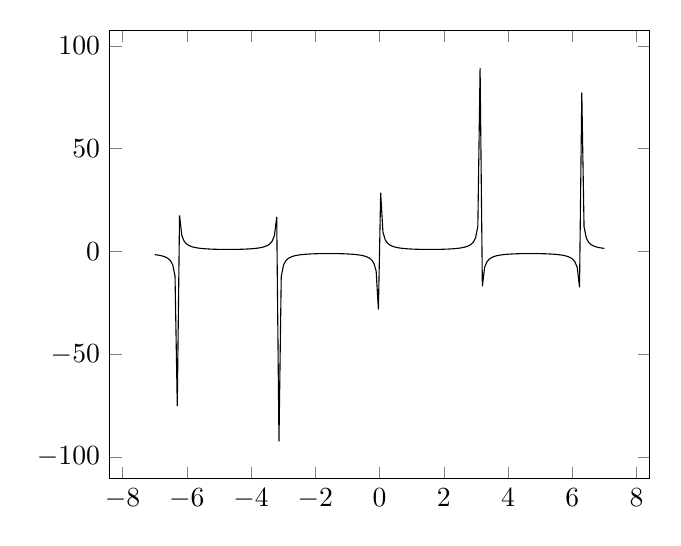
\begin{tikzpicture}
    \begin{axis}
      \addplot[samples=200,domain=-7:7]{1/sin(deg(x))};
    \end{axis}
\end{tikzpicture}
\end{image}

\begin{callout}
  {\bf Note:} the vertical lines in the above picture are not part of the graph of $y=\csc(x)$. They represent the vertical asymptotes for the graph. We will discuss asymptotes in more detail in the next couple of units.
\end{callout}

\end{example}

\begin{exploration} Repeat the discussion made above for the secant and cotangent functions. Namely:
  \begin{enumerate}[label=\alph*.]
  \item For which values of $x$ do we have that $\cos x = 0$? And for which values of $x$ do we have $\tan x = 0$?  
  \item For which values of $x$ is $\sec(x)$ undefined? And for which values o $x$ is $\cot(x)$ undefined?
  \end{enumerate}
\end{exploration}


\begin{callout}
  {\bf Warning:} Do not confuse reciprocals of trigonometric functions, as discussed above, with inverse trigonometric functions such as $\arcsin$, $\arccos$ and $\arctan$ (as in ``inverse functions'', as discussed in Section 3-2).
\end{callout}


%\typeout{************************************************}
%\typeout{Summary}
%\typeout{************************************************}

\begin{summary}\begin{itemize}
\item The function $f(x) = 1/x$ is defined for all non-zero values of $x$. It is an odd function, and its asymptotics can be understood by its graph, called a \emph{hyperbola}.
\item We can compose $f(x) = 1/x$ with functions we frequently encounter, to produce new functions which may prove useful when modeling certain problems and real life situations. For instance, doing this to trigonometric functions, one obtains $$   \csc x = \frac{1}{\sin x}, \quad \sec x = \frac{1}{\cos x} \quad\mbox{and} \quad \cot x = \frac{1}{\tan x}.  $$They are called, respectively, the \emph{cosecant}, \emph{secant} and \emph{cotangent} functions.
\end{itemize}\end{summary}




\end{document}
